\documentclass[tikz,border=10pt]{standalone}
\usepackage{tikz}
\usetikzlibrary{positioning,arrows.meta,fit,backgrounds,calc,shapes.multipart}

\begin{document}
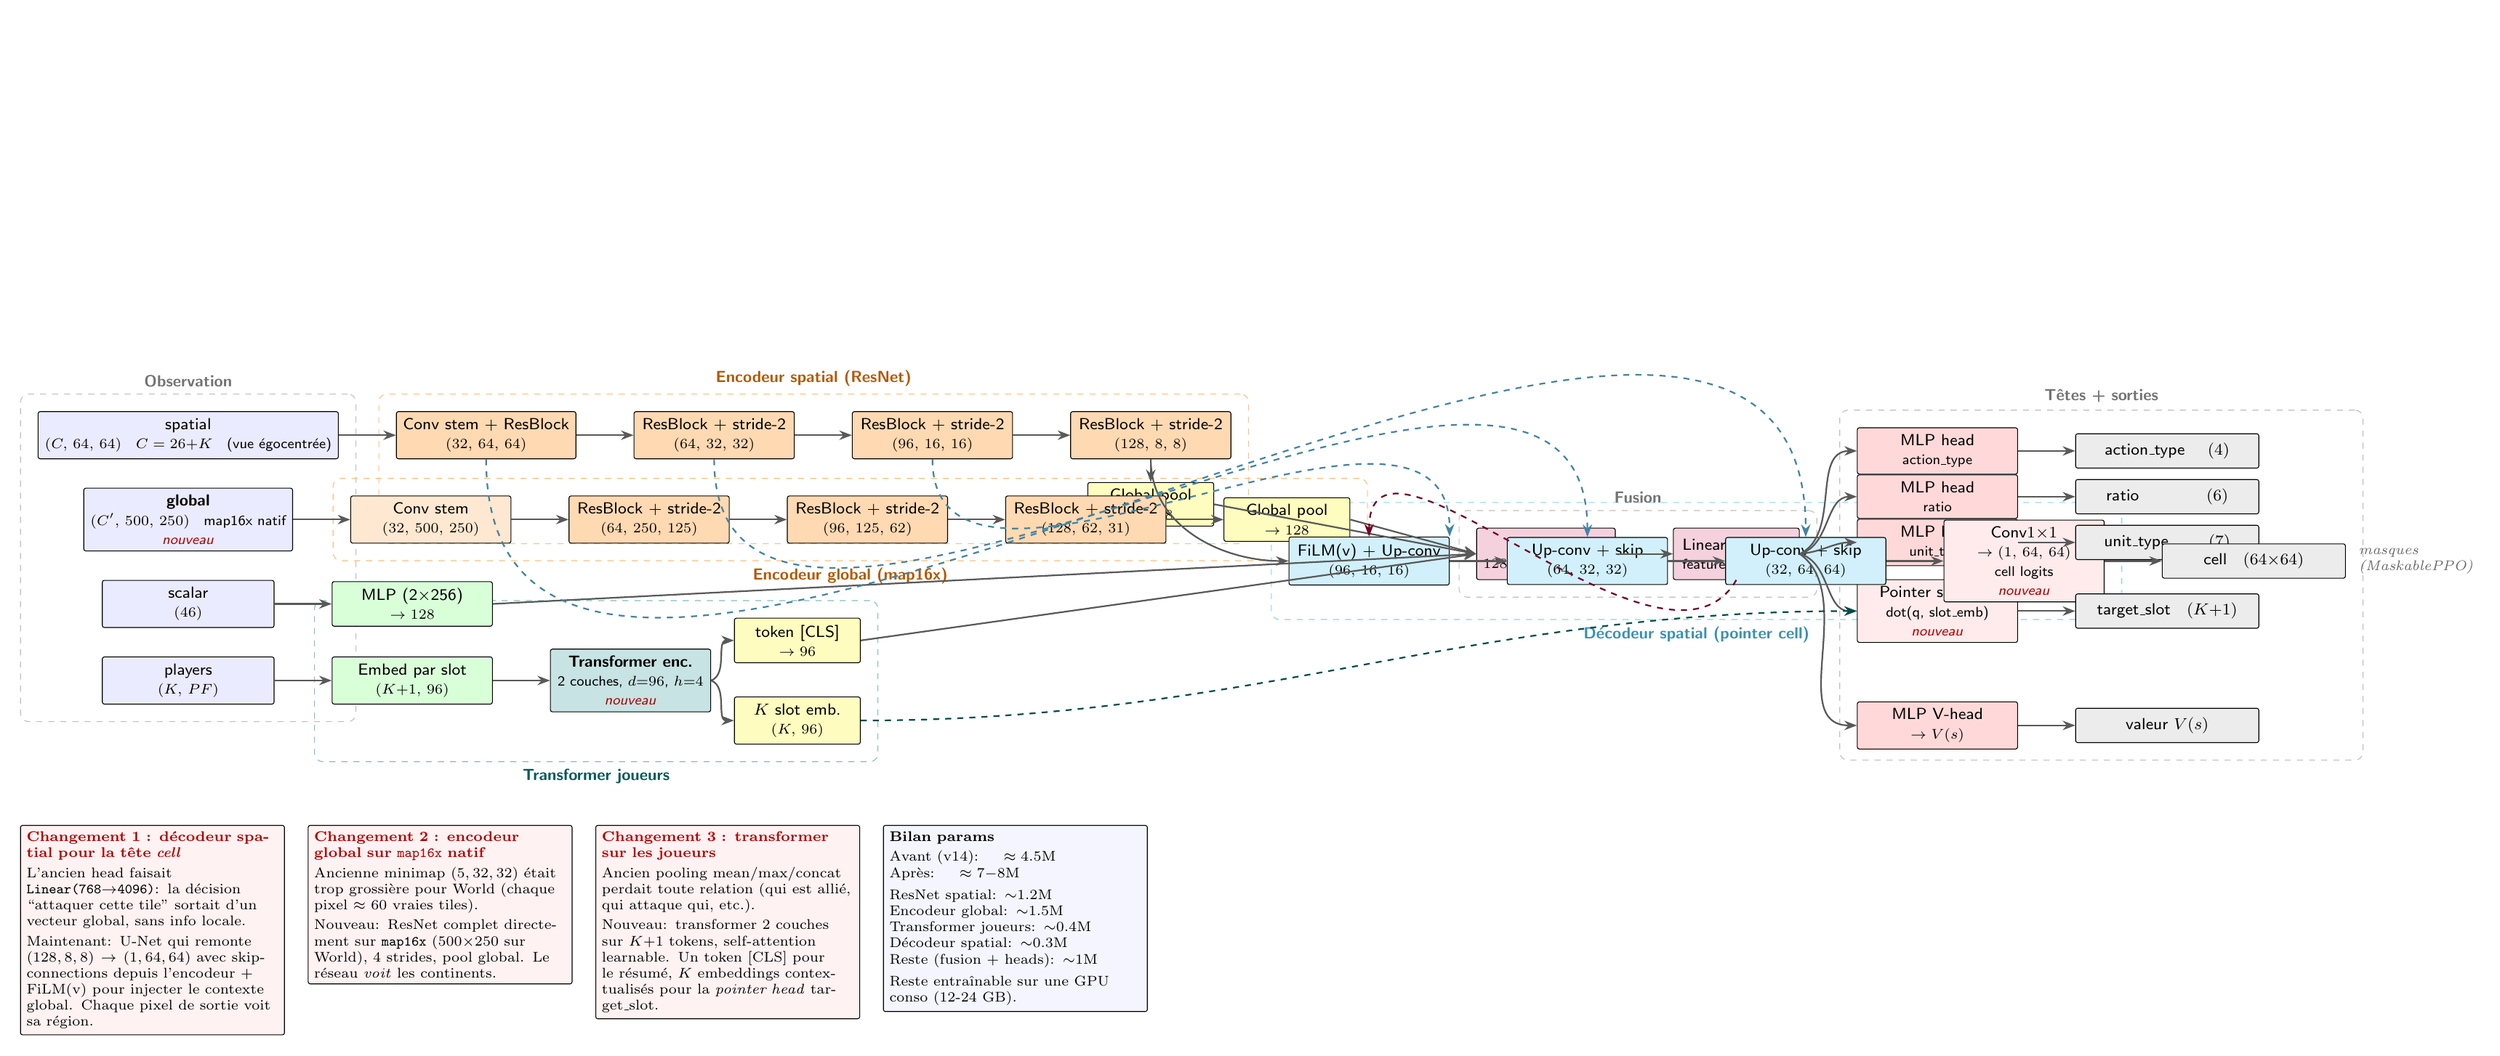
\begin{tikzpicture}[
  font=\sffamily\footnotesize,
  >={Stealth[length=2.2mm]},
  node distance=5mm and 10mm,
  input/.style   ={draw, rounded corners=1pt, fill=blue!8,   minimum width=30mm, minimum height=8mm, align=center},
  cnn/.style     ={draw, rounded corners=1pt, fill=orange!18, minimum width=28mm, minimum height=7mm, align=center},
  res/.style     ={draw, rounded corners=1pt, fill=orange!30, minimum width=28mm, minimum height=7mm, align=center},
  dec/.style     ={draw, rounded corners=1pt, fill=cyan!18,   minimum width=28mm, minimum height=7mm, align=center},
  mlp/.style     ={draw, rounded corners=1pt, fill=green!15,  minimum width=28mm, minimum height=7mm, align=center},
  tr/.style      ={draw, rounded corners=1pt, fill=teal!22,   minimum width=28mm, minimum height=7mm, align=center},
  pool/.style    ={draw, rounded corners=1pt, fill=yellow!25, minimum width=22mm, minimum height=6mm, align=center},
  fuse/.style    ={draw, rounded corners=1pt, fill=purple!18, minimum width=22mm, minimum height=9mm, align=center},
  head/.style    ={draw, rounded corners=1pt, fill=red!15,    minimum width=28mm, minimum height=7mm, align=center},
  outbox/.style  ={draw, rounded corners=1pt, fill=gray!15,   minimum width=32mm, minimum height=6mm, align=center},
  legend/.style  ={draw, rounded corners=1pt, fill=blue!4, minimum width=46mm, text width=44mm, align=left,
                   font=\scriptsize, inner sep=3pt},
  dim/.style     ={font=\scriptsize\itshape, text=black!60},
  arr/.style     ={->, thick, black!65},
  skip/.style    ={->, dashed, thick, cyan!60!black},
  newbox/.style  ={fill=red!8},
]

% ============================================================
% INPUTS (gauche)
% ============================================================
\node[input] (ispa)                   {spatial \\ \scriptsize $(C,\,64,\,64)$ \; $C=26{+}K$ \; (vue \'egocentr\'ee)};
\node[input, below=of ispa] (iglo)    {\textbf{global} \\ \scriptsize $(C',\,500,\,250)$ \; map16x natif \\ \scriptsize \textcolor{red!70!black}{\emph{nouveau}}};
\node[input, below=of iglo] (isca)    {scalar \\ \scriptsize $(46)$};
\node[input, below=of isca] (ipla)    {players \\ \scriptsize $(K,\,PF)$};

% ============================================================
% BRANCHE SPATIALE (CNN encoder + U-Net decoder)
% ============================================================
\node[res, right=of ispa] (se1)       {Conv stem + ResBlock \\ \scriptsize $(32,\,64,\,64)$};
\node[res, right=of se1]  (se2)       {ResBlock + stride-2 \\ \scriptsize $(64,\,32,\,32)$};
\node[res, right=of se2]  (se3)       {ResBlock + stride-2 \\ \scriptsize $(96,\,16,\,16)$};
\node[res, right=of se3]  (se4)       {ResBlock + stride-2 \\ \scriptsize $(128,\,8,\,8)$};

% Pool global pour la fusion
\node[pool, below=4mm of se4] (sgap)  {Global pool \\ \scriptsize $\rightarrow 128$};

% ============================================================
% BRANCHE GLOBALE (map16x, encodeur profond pool\'e)
% ============================================================
\node[cnn, right=of iglo]           (g1) {Conv stem \\ \scriptsize $(32,\,500,\,250)$};
\node[res, right=of g1]             (g2) {ResBlock + stride-2 \\ \scriptsize $(64,\,250,\,125)$};
\node[res, right=of g2]             (g3) {ResBlock + stride-2 \\ \scriptsize $(96,\,125,\,62)$};
\node[res, right=of g3]             (g4) {ResBlock + stride-2 \\ \scriptsize $(128,\,62,\,31)$};
\node[pool, right=of g4]            (gp) {Global pool \\ \scriptsize $\rightarrow 128$};

% ============================================================
% BRANCHE SCALAIRE
% ============================================================
\node[mlp, right=of isca] (sm)       {MLP (2$\times$256) \\ \scriptsize $\rightarrow 128$};

% ============================================================
% BRANCHE JOUEURS (transformer)
% ============================================================
\node[mlp, right=of ipla]  (pe)      {Embed par slot \\ \scriptsize $(K{+}1,\,96)$};
\node[tr,  right=of pe]    (tr)      {\textbf{Transformer enc.} \\ \scriptsize 2 couches, $d{=}96$, $h{=}4$ \\ \scriptsize \textcolor{red!70!black}{\emph{nouveau}}};
\node[pool, right=4mm of tr, yshift=7mm]  (cls)   {token [CLS] \\ \scriptsize $\rightarrow 96$};
\node[pool, right=4mm of tr, yshift=-7mm] (slots) {$K$ slot emb. \\ \scriptsize $(K,\,96)$};

% ============================================================
% FUSION
% ============================================================
\node[fuse, right=22mm of gp, yshift=-6mm] (concat) {Concat \\ \scriptsize $128{+}128{+}128{+}96$};
\node[fuse, right=of concat]               (fuse)   {Linear + ReLU \\ \scriptsize features $v = 512$};

% ============================================================
% T\^ETES
% ============================================================
% T\^etes "simples" issues du vecteur global v
\node[head, right=of fuse, yshift=18mm] (hat) {MLP head \\ \scriptsize action\_type};
\node[head, right=of fuse, yshift=10mm] (hra) {MLP head \\ \scriptsize ratio};
\node[head, right=of fuse, yshift=2mm]  (hun) {MLP head \\ \scriptsize unit\_type};

% target\_slot: pointer sur les slot embeddings (dot-product)
\node[head, right=of fuse, yshift=-10mm, newbox] (hts) {Pointer sur slots \\ \scriptsize dot(q, slot\_emb) \\ \scriptsize \textcolor{red!70!black}{\emph{nouveau}}};

% Spatial decoder (U-Net) pour le cell head
\node[dec, right=of se4, yshift=-22mm]  (d1)  {FiLM(v) + Up-conv \\ \scriptsize $(96,\,16,\,16)$};
\node[dec, right=of d1]                 (d2)  {Up-conv + skip \\ \scriptsize $(64,\,32,\,32)$};
\node[dec, right=of d2]                 (d3)  {Up-conv + skip \\ \scriptsize $(32,\,64,\,64)$};
\node[head, right=of d3, newbox]        (hcell) {Conv$1{\times}1$ \\ \scriptsize $\rightarrow (1,\,64,\,64)$ \\ \scriptsize cell logits \\ \scriptsize \textcolor{red!70!black}{\emph{nouveau}}};

% V-head
\node[head, right=of fuse, yshift=-30mm] (vhd) {MLP V-head \\ \scriptsize $\rightarrow V(s)$};

% ============================================================
% SORTIES
% ============================================================
\node[outbox, right=of hat] (oat) {action\_type \quad $(4)$};
\node[outbox, right=of hra] (ora) {ratio \qquad\quad\; $(6)$};
\node[outbox, right=of hun] (oun) {unit\_type \qquad $(7)$};
\node[outbox, right=of hts] (ots) {target\_slot \; $(K{+}1)$};
\node[outbox, right=of hcell, align=center] (ocell) {cell \; $(64{\times}64)$};
\node[outbox, right=of vhd] (ov)  {valeur $V(s)$};

% ============================================================
% AR\^ETES
% ============================================================
% Branche spatiale: cha\^ine d'encodeur
\draw[arr] (ispa) -- (se1);
\draw[arr] (se1)  -- (se2);
\draw[arr] (se2)  -- (se3);
\draw[arr] (se3)  -- (se4);
\draw[arr] (se4)  -- (sgap);

% Branche globale
\draw[arr] (iglo) -- (g1);
\draw[arr] (g1)   -- (g2);
\draw[arr] (g2)   -- (g3);
\draw[arr] (g3)   -- (g4);
\draw[arr] (g4)   -- (gp);

% Branche scalaire
\draw[arr] (isca) -- (sm);

% Branche joueurs
\draw[arr] (ipla) -- (pe);
\draw[arr] (pe)   -- (tr);
\draw[arr] (tr.east) to[out=20,in=180]  (cls.west);
\draw[arr] (tr.east) to[out=-20,in=180] (slots.west);

% Concat
\foreach \n in {sgap, gp, sm, cls}
  \draw[arr] (\n.east) -- (concat.west);
\draw[arr] (concat) -- (fuse);

% Vecteur global v vers t\^etes "simples"
\draw[arr] (fuse.east) to[out=25,in=180]  (hat.west);
\draw[arr] (fuse.east) to[out=15,in=180]  (hra.west);
\draw[arr] (fuse.east) to[out=5,in=180]   (hun.west);
\draw[arr] (fuse.east) to[out=-15,in=180] (hts.west);
\draw[arr] (fuse.east) to[out=-35,in=180] (vhd.west);

% target_slot: pointer sur slot embeddings
\draw[arr, dashed, teal!60!black] (slots.east) to[out=0,in=180] (hts.west);

% Spatial decoder: lire les features (8,8) + skips de l'encodeur
\draw[arr] (se4.south) to[out=-90,in=180] (d1.west);
% FiLM : v module le decoder
\draw[arr, dashed, purple!60!black] (fuse.south) to[out=-120,in=90] (d1.north);
\draw[arr] (d1) -- (d2);
\draw[arr] (d2) -- (d3);
\draw[arr] (d3) -- (hcell);

% Skip connections U-Net
\draw[skip] (se3.south) to[out=-90,in=90] (d1.north east);
\draw[skip] (se2.south) to[out=-90,in=90] (d2.north);
\draw[skip] (se1.south) to[out=-90,in=90] (d3.north);

% Sorties
\draw[arr] (hat) -- (oat);
\draw[arr] (hra) -- (ora);
\draw[arr] (hun) -- (oun);
\draw[arr] (hts) -- (ots);
\draw[arr] (hcell) -- (ocell);
\draw[arr] (vhd) -- (ov);

% ============================================================
% MASQUES (annotation)
% ============================================================
\node[dim, right=1mm of ocell, align=left]
  {\scriptsize masques\\ \scriptsize (MaskablePPO)};

% ============================================================
% GROUPES
% ============================================================
\begin{scope}[on background layer]
  \node[draw=black!25, dashed, rounded corners, inner sep=3mm,
        fit=(ispa)(ipla), label={[black!55]above:\textbf{Observation}}] (obsgrp) {};
  \node[draw=orange!50, dashed, rounded corners, inner sep=3mm,
        fit=(se1)(se4)(sgap),
        label={[orange!70!black]above:\textbf{Encodeur spatial (ResNet)}}] (encgrp) {};
  \node[draw=cyan!50, dashed, rounded corners, inner sep=3mm,
        fit=(d1)(d3)(hcell),
        label={[cyan!70!black]below:\textbf{D\'ecodeur spatial (pointer cell)}}] (decgrp) {};
  \node[draw=teal!50, dashed, rounded corners, inner sep=3mm,
        fit=(pe)(tr)(cls)(slots),
        label={[teal!70!black]below:\textbf{Transformer joueurs}}] {};
  \node[draw=orange!50, dashed, rounded corners, inner sep=3mm,
        fit=(g1)(g4)(gp),
        label={[orange!70!black]below:\textbf{Encodeur global (map16x)}}] {};
  \node[draw=black!25, dashed, rounded corners, inner sep=3mm,
        fit=(concat)(fuse), label={[black!55]above:\textbf{Fusion}}] {};
  \node[draw=black!25, dashed, rounded corners, inner sep=3mm,
        fit=(hat)(ov)(oat)(ocell), label={[black!55]above:\textbf{T\^etes + sorties}}] {};
\end{scope}

% ============================================================
% L\'EGENDE (bas) : rappel des 3 changements structurels
% ============================================================
\node[legend, below=18mm of obsgrp.south west, anchor=north west, fill=red!5]
  (lega) {%
  \textbf{\textcolor{red!70!black}{Changement 1 : d\'ecodeur spatial pour la t\^ete \textit{cell}}}\\[2pt]
  \scriptsize L'ancien head faisait \texttt{Linear(768$\to$4096)}: la d\'ecision ``attaquer cette tile'' sortait d'un vecteur global, sans info locale.\\[2pt]
  \scriptsize Maintenant: U-Net qui remonte $(128,8,8) \to (1,64,64)$ avec skip-connections depuis l'encodeur + FiLM(v) pour injecter le contexte global. Chaque pixel de sortie voit sa r\'egion.
  };
\node[legend, right=4mm of lega.north east, anchor=north west, fill=red!5]
  (legb) {%
  \textbf{\textcolor{red!70!black}{Changement 2 : encodeur global sur \texttt{map16x} natif}}\\[2pt]
  \scriptsize Ancienne minimap $(5,32,32)$ \'etait trop grossi\`ere pour World (chaque pixel $\approx$ 60 vraies tiles).\\[2pt]
  \scriptsize Nouveau: ResNet complet directement sur \texttt{map16x} ($500{\times}250$ sur World), 4 strides, pool global. Le r\'eseau \emph{voit} les continents.
  };
\node[legend, right=4mm of legb.north east, anchor=north west, fill=red!5]
  (legc) {%
  \textbf{\textcolor{red!70!black}{Changement 3 : transformer sur les joueurs}}\\[2pt]
  \scriptsize Ancien pooling mean/max/concat perdait toute relation (qui est alli\'e, qui attaque qui, etc.).\\[2pt]
  \scriptsize Nouveau: transformer 2 couches sur $K{+}1$ tokens, self-attention learnable. Un token [CLS] pour le r\'esum\'e, $K$ embeddings contextualis\'es pour la \textit{pointer head} target\_slot.
  };
\node[legend, right=4mm of legc.north east, anchor=north west]
  (legd) {%
  \textbf{Bilan params}\\[2pt]
  \scriptsize Avant (v14): \;\; $\approx 4.5$M \\
  \scriptsize Apr\`es: \;\; $\approx 7{-}8$M \\[3pt]
  \scriptsize ResNet spatial: $\sim$1.2M \\
  \scriptsize Encodeur global: $\sim$1.5M \\
  \scriptsize Transformer joueurs: $\sim$0.4M \\
  \scriptsize D\'ecodeur spatial: $\sim$0.3M \\
  \scriptsize Reste (fusion + heads): $\sim$1M \\[3pt]
  \scriptsize Reste entra\^inable sur une GPU conso (12-24 GB).
  };

\end{tikzpicture}
\end{document}
